% This is sigproc-sp.tex -FILE FOR V2.6SP OF ACM_PROC_ARTICLE-SP.CLS
% OCTOBER 2002
%
% It is an example file showing how to use the 'acm_proc_article-sp.cls' V2.6SP
% LaTeX2e document class file for Conference Proceedings submissions.
% ----------------------------------------------------------------------------------------------------------------
% This .tex file (and associated .cls V2.6SP) *DOES NOT* produce:
%       1) The Permission Statement
%       2) The Conference (location) Info information
%       3) The Copyright Line with ACM data
%       4) Page numbering
%
%  However, both the CopyrightYear (default to 2002) and the ACM Copyright Data
% (default to X-XXXXX-XX-X/XX/XX) can still be over-ridden by whatever the author
% inserts into the source .tex file.
% e.g.
% \CopyrightYear{2003} will cause 2003 to appear in the copyright line.
% \crdata{0-12345-67-8/90/12} will cause 0-12345-67-8/90/12 to appear in the copyright line.
%
% ---------------------------------------------------------------------------------------------------------------
% It is an example which *does* use the .bib file (from which the .bbl file
% is produced).
% REMEMBER HOWEVER: After having produced the .bbl file,
% and prior to final submission,
% you need to 'insert'  your .bbl file into your source .tex file so as to provide
% ONE 'self-contained' source file.
%
% Questions regarding SIGS should be sent to
% Adrienne Griscti ---> griscti@acm.org
%
% Questions/suggestions regarding the guidelines, .tex and .cls files, etc. to
% Gerald Murray ---> murray@acm.org 
%
% For tracking purposes - this is V2.6SP - OCTOBER 2002

\documentclass[12pt]{article}
\setlength{\oddsidemargin}{0in}
\setlength{\evensidemargin}{0in}
\setlength{\topmargin}{0in}
\setlength{\headheight}{0in}
\setlength{\headsep}{0in}
\setlength{\textwidth}{6in}
\setlength{\textheight}{9in}
\setlength{\parindent}{0in} 

\usepackage{graphicx} %For jpg figure inclusion
\usepackage{times} %For typeface
\usepackage{epsfig}
\usepackage{color} %For Comments
\usepackage[all]{xy}
\usepackage{float}
\usepackage{subfigure} 
\usepackage{hyperref}
\usepackage{url}
\usepackage{parskip}
%\usepackage[style=numeric,backend=biber]{biblatex}



%% Elena's favorite green (thanks, Fernando!)
\definecolor{ForestGreen}{RGB}{34,139,34}
\definecolor{MaxBlue}{RGB}{62,65,198}
% Uncomment this if you want to show work-in-progress comments
\newcommand{\comment}[1]{{\bf \tt  {#1}}}
% Uncomment this if you don't want to show comments
%\newcommand{\comment}[1]{}
\newcommand{\emcomment}[1]{\textcolor{ForestGreen}{\comment{Elena: {#1}}}}
\newcommand{\mmcomment}[1]{\textcolor{MaxBlue}{\comment{Max: {#1}}}}
\newcommand{\todo}[1]{\textcolor{blue}{\comment{To Do: {#1}}}}
\newcommand{\code}[1]{{\texttt {#1}}}



\begin{document}
\pagestyle{plain}
%
% --- Author Metadata here ---
%\conferenceinfo{WOODSTOCK}{'97 El Paso, Texas USA}
%\setpagenumber{50}
%\CopyrightYear{2002} % Allows default copyright year (2002) to be
%over-ridden - IF NEED BE. 
%\crdata{0-12345-67-8/90/01}  % Allows default copyright data
%(X-XXXXX-XX-X/XX/XX) to be over-ridden. 
% --- End of Author Metadata ---




\title{Adopting Node.js and CoffeeScript in a Software Design Course}
%\subtitle{[Extended Abstract \comment{DO WE NEED THIS?}]
%\titlenote{}}
%
% You need the command \numberofauthors to handle the "boxing"
% and alignment of the authors under the title, and to add
% a section for authors number 4 through n.
%
% Up to the first three authors are aligned under the title;
% use the \alignauthor commands below to handle those names
% and affiliations. Add names, affiliations, addresses for
% additional authors as the argument to \additionalauthors;
% these will be set for you without further effort on your
% part as the last section in the body of your article BEFORE
% References or any Appendices.




\author{
Maxwell Marti \\
%Computer Science Discipline \\
University of Minnesota Morris\\
Morris, MN 56267\\
mart2967@morris.umn.edu
}




\date{}




\maketitle
\thispagestyle{empty}


\section*{\centering Abstract}
Overhauling the contents of any computer science course is a formidable undertaking, especially when the class is based on cutting-edge software development techniques.
The Software Design and Development course at the University of Minnesota, Morris is focused on collaboration, with students working on a project for a customer, this year a private company. 
The course recently transitioned from web development with Groovy and Grails to a more modern approach with Node.js and CoffeeScript.
Node.js has risen into prominence for its unique properties, such as server-side JavaScript, non-blocking I/O, extendability, and native web-serving. 
CoffeeScript is a language designed to improve upon JavaScript, while being universally compatible with JavaScript-based tools. 
Concepts including agile development, thick-client systems, testing, version control, and continuous integration will be covered. 
I will give an overview of the development environment and collaboration structure used by the students. 
I will conclude with an analysis of this new approach.



\newpage
%this causes problems when compiling.

\setcounter{page}{1}


\section{Introduction}\label{sec:introduction}
\subsection{Course Background}\label{sec:course_background}
The Software Design and Development course is a project-based course, with students collaborating throughout the semester to build one piece of software for a customer. 
The students work in teams of at least four, working on one aspect of the project for the span of an iteration, typically two weeks. 
At the end of each iteration, the teams give presentations to the customer; this could either be a faculty member or a real company, this year's being the latter. 
As the semester progresses, the disparate codebases are assembled and improved by teams of increasing size, resulting in two or three large projects that must be consolidated into a final product. 
The development process utilizes the agile methodology, with the class holding group event such as the Inception deck, where the project is unveiled and students brainstorm ideas for how to build it. 
A key part of agile development is the user story, which is a description of some action a user may want to perform, such as logging in or "liking" a piece of content. 
Once students have created their stories, the customer selects which ones will be the focus of the iteration. Stories can be compared to a main ``to-do'' list for the project. 
By focusing on user interactions instead of technical specifications, the agile process is more responsive to any changes in the project's scope than other methods, and allows flexibility in how developers choose to implement features.



\subsection{Reasons for Transition}\label{sec:reasons_for_transition}
The course has historically been taught using different technologies, most recently the Grails framework for web applications, and Java with the Swing library before that. 
The transition from a heavily server-reliant technology like Grails to a more lightweight technology was driven by the state of cutting-edge web development practices. 
More and more real-world web applications are being built with client-side JavaScript frameworks that handle more tasks and ease the burden on the central server. 
These frameworks include Backbone.js, Angular.js, Ember.js, and many more. 
They typically do not make any assumptions about the server, other than that it can accept REST-style HTTP requests. 
REST is short for Representational State Transfer, and REST-style applications are those that do not require the client to know anything about how to interact with the API, therefore telling the client what they want and where to send it. 
The standard used to communicate with the API is HTTP requests such as GET and POST.

Well designed systems have their URL structure standardized. 
Node in particular uses JSON to pass data back and forth. 
JSON stands for JavaScript Object Notation, and describes objects as nested key-value pairs. 
One benefit of using JavaScript on the client and the server is the ease of communication between them using JSON. 
All these properties leave the developer free to choose their tools without fear of incompatibilities. 

The adoption of client-side JavaScript frameworks has been accelerated by both the increasing power of internet capable-devices, and the potential increased load on back-end servers due to their rapid proliferation. 
One goal of the Software Design course is to simulate a real work environment, preparing students for the kinds of projects they are likely to see in their careers. 
We chose to adopt this new paradigm as it has become popular in the professional sphere, as well as for its very customizable nature.


\subsection{The Development Environment}\label{sec:IDE}
\begin{figure}[h!]
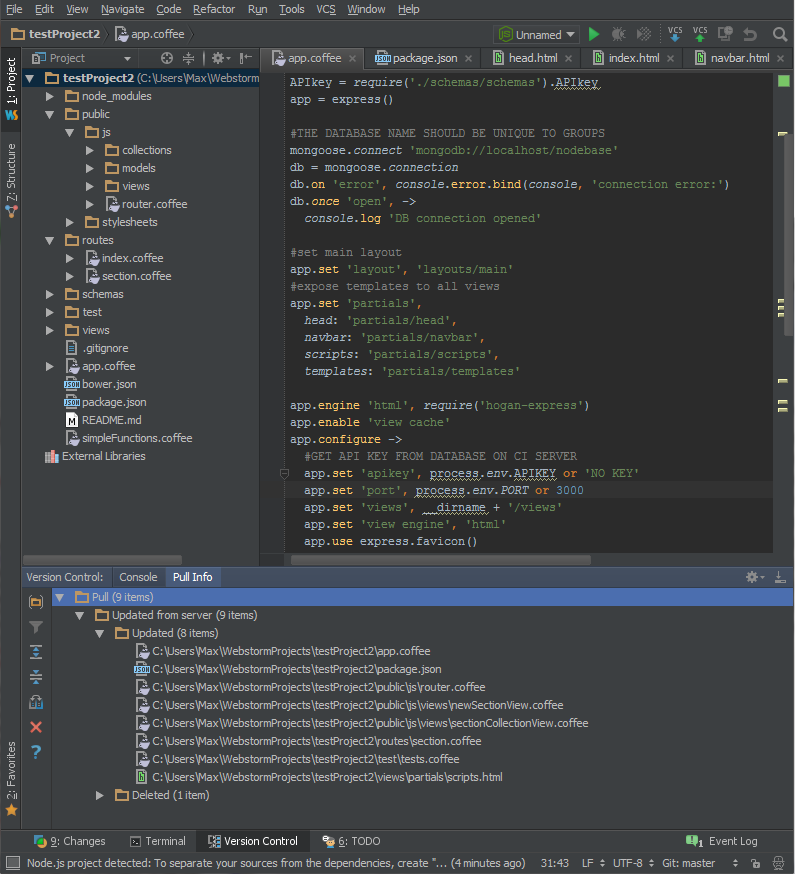
\includegraphics[width=\linewidth]{img/webstorm.png}
\caption{WebStorm using the dark theme, demonstrating CoffeeScript syntax highlighting and recent version control changes}
\end{figure}
Selecting the development tools is a crucial part of any project. 
To use a full Integrated Development Environment or a collection of more lightweight tools is an important decision. 
It was decided to use WebStorm~\cite{WebStorm}, an IDE based on the IntelliJ IDEA program. 
The developer offers a free educational license, which was used for all class activities. 
The IDE itself offers a well-designed user interface, with file management, tabs, and built-in terminal windows. 
It offers robust support for JavaScript and Node.js, as well as various test frameworks, code coverage tools, and package management. 
It supports various version control systems, including Git. 
It also has support for enhanced package management with \code{npm}, the package manager that ships with Node.js. 
As of the latest version, similar features have been released for \code{bower}, a module for front-end packages like jOuery.

\subsection{Project Structure}\label{sec:structure}
The core architecture of the project must be well defined before starting any serious development, so in the weeks preceding the start of the course, we chose a set of tools and planned the general layout of the project. 
Because the students would be building a web application, a strong distinction between server code and client code was needed, especially since the same language is used on both ends. 
The Node.js based server would be backed with a database, and be able to do basic HTML templating so as to reduce code duplication. 
On the client, the constructed templates sent by the server are populated with the relevant content via our JavaScript framework, and upon changing states or navigating through the site, it will only download the needed data instead of requesting a pre-rendered page from the server. 
This structure allows us to separate the data operations from the construction of HTML, providing code that can easily be reused in different areas of the application.

\section{The Server}\label{sec:server}
The project setup will be described in two sections, covering the server- and client-side technologies. 
The server used in this project is responsible for taking HTTP requests, routing them to the proper functions, and returning a response. 
The server contains less logic than in other systems, as most of the rendering and light data manipulation is left up to the client. 
This leaves it free to focus on providing an API that performs operations and handles requests with the backing of its database.

\subsection{Node.js}\label{sec:node}
For the core of the server, Node.js~\cite{Node} was chosen. 
Node is a platform built for web application development, running on the V8 JavaScript engine found in Google Chrome. 
In contrast to traditional web servers, Node does not use threads to manage concurrent connections; instead, when a user connects, a JavaScript callback is triggered that performs the requested operation. 
Node uses non-blocking I/O to ensure that the server never hangs on a request and all users are served as soon as possible. 
The system is called an event loop, meaning that Node is always looping, listening for events and delegating them to their appropriate functions when triggered. 
This is similar to how a web browser handles events like clicks, hovers, changes, and button presses. 

Node has a massive ecosystem of plugins, called modules, that allow developers to easily add or integrate functionality they desire. 
Modules are installed with \code{npm} (stands for ``node package manager''), the package manager that ships with Node. 
Some of the modules used in the course are detailed below.

\subsubsection{Express}\label{sec:express}
Express~\cite{Express} is a node module that adds a more robust framework to Node for building web applications. 
It handles many common operations, allows advanced configuration of the server, and breaks up the logic into multiple areas.  
For example, it simplifies the definition of API routes, defining static files directories, setting global variables, and much more. 
It is designed to not force developers into one type of application structure, and as a result, Express applications can take many forms.

\subsection{Hogan}\label{sec:hogan}
While most of the rendering takes place on the client, it is useful to construct a lightweight HTML template that our front-end JavaScript framework can then insert content into. 
Hogan.js~\cite{Hogan} is a templating engine from Twitter, based on the Mustache.js specification. 
It has improved runtime on many operations which is why we selected it from the large amount of templating engines available.
\begin{verbatim}
<html>
	<head>
{{> head_content}} <!-- These kind of tags indicate a partial -->
</head>
<body>
{{> navbar}} 
    <div class="container">
        {{{ yield }}} <!-- Where the page skeleton will go -->
    </div>
{{> scripts}}
</body>
</html>
\end{verbatim}
Partials are independent HTML files that have some data that needs to be included on the page but may be reused in other pages. 
Here the head, navbar, and deferred scripts are loaded in to the main template.

\subsection{CoffeeScript}\label{sec:coffee}
While Node.js applications are natively written in JavaScript, a language called CoffeeScript~\cite{CoffeeScript} is used in the course. 
CoffeeScript is a language with syntax inspired by Python, Ruby, and Haskell that transpiles to JavaScript. 
To transpile is to convert a high-level language into another high level language, whereas compiling converts to a lower-level language. 
The goal of Coffeescript is to make JavaScript easier to read and write. 
It accomplishes this goal by abstracting over the often unnecessarily complex conventions of JavaScript. 
A typical CoffeeScript file is approximately one-third shorter than the equivalent JavaScript file. 
It also includes features that remove the often-unexpected nature of the JavaScript scope, automatically using the \code{var} keyword where it is needed. 
Common JavaScript scope pitfalls include accidentally creating or overwriting a global variable, improperly binding variables to a \code{this} object, and many more. 
CoffeeScript defaults to much more clear and robust code. 
Below is a sample of CoffeeScript syntax taken from the official site.
\begin{verbatim}
# Conditions:
number = -42 if opposite

# Functions:
square = (x) -> x * x
alert square 3

# Arrays:
list = [1, 2, 3, 4, 5]

# Objects:
math =
  root:   Math.sqrt
  square: square
  cube:   (x) -> x * square x

# Existence:
alert "I knew it!" if elvis?

\end{verbatim}
CoffeeScript is similar to Python in that indentation is a part of syntax: each level of indentation corresponds to a level of code nesting. 
Thus braces or other structuring elements are not needed.
The "backwards" \code{if} statements are intended to help with short operations such as assignment, while the traditional structure is used for complex conditionals. 
Parentheses are not needed on function calls unless there is a need for clear nesting. 
The symbol \code{->} is equivalent to JavaScript keyword \code{function} for function definitions. 
Parameters are given in parentheses preceding the arrow. 
Functions may be named or anonymous. 


\subsection{MongoDB}\label{sec:mongo}
Most serious web applications need a database, and MongoDB~\cite{MongoDB} is a great fit for a Node-based project. 
It stores data in JavaScript Object Notation, or JSON. This allows queries to return data that is immediately useful to the application, whereas a more traditional SQL based database might require a hefty function to parse and organize the data. 
Queries are also written in JavaScript. The technology is known for its  load balancing features, which allow one database to run across multiple machines (this is known as sharding); however, the scale of our project is not large enough to take advantage of these features.

\subsubsection{Mongoose}\label{sec:mongoose}
Mongoose~\cite{Mongoose} is a Node module that simplifies and enhances interaction with MongoDB. 
It offers the ability to define database schemas, and query the database based on the models one has defined. 
It simplifies working with the data by integrating model validation, type casting, and query building for improved ease of development. 
Below is an example of an edit function on the server, written in CoffeeScript.
\begin{verbatim}
exports.edit = (req, res) ->
  section = req.body
  delete section._id
  id = req.params.id
  Section.update { _id: id },
  { $set: section },
  (err, numAffected, raw) ->
    console.log err if err
    console.log '%d document updated', numAffected
    console.log 'The raw response from Mongo was ', raw
    res.send section
\end{verbatim}
In this code, incoming data is read from the HTTP request, and the function \code{update} is called on the Mongoose database collection called Section. 
This function updates a piece of data by its \code{id}.


\section{The Client}\label{sec:client}
The client refers to all the code written to run directly on the user's web browser. 
On initial page load, the server sends all the necessary JavaScript files to the client, which then handles layout, rendering of data to HTML, user interaction and event handling, and more. 
This client-side JavaScript handles many functions that were once the domain of the server, and by doing so allows the latter to focus on data operations.

\subsection{jQuery}\label{sec:jquery}
A mainstay in the web development world, jQuery~\cite{jQuery} is a JavaScript library that offers simplified scripting and interaction with HTML. 
The core of jQuery is the selector engine, which allows lookup, traversal, and manipulation of the Document Object Model (DOM) that makes up the heart of any web page. 
The other systems on the client use jQuery functions to enhance their own abilities. Some simple jQuery operations are shown below.
\begin{verbatim}
// set html for element
$("p:first" ).html( "This is the <em>first</em> paragraph");

// set value for all inputs of myClass
$("input.myClass").val("default text");

// bind a function to the click event of an element
$("#myButton").on("click", function(){
    alert("Button was clicked");
});
\end{verbatim}
The \code{\$( )} syntax denotes a jQuery object, which is given the value of the selector inside of it. 
Elements can be selected by \code{id} with \code{\$("\#someDiv")}, and by \code{class} with \code{\$(".someClass")}.
Functions can then be called on them and range from the simple, such as \code{hide()}, which hides the selected element(s), to more advanced ones, such as binding event listeners to an object that act on things like mouse clicks.


\subsection{Backbone.js}\label{sec:backbone}
Backbone.js~\cite{Backbone} is a JavaScript framework for creating Single-Page Applications (SPAs). 
These are web pages that do not reload the whole page when navigating to another part of the site. 
Instead, the necessary data is loaded from the server, and the relevant portion of the page is re-rendered using JavaScript. 
Backbone provides a structure and set of functionality for defining the operation of a site. 
A stated goal of Backbone is that it does not make many design decisions; these are left up to the developer. 
This approach is a good one for a classroom environment as students are able to learn more about proper application design. 
Backbone provides classes for Models, Views, Collections, and Routers. 
This provides a variation on the common Model-View-Controller pattern, where data storage (model), business logic (controller) and content rendering (view) are separated into distinct components. 
Backbone does not adhere strictly to this model, sharing the responsibility of the controller across the Router and Views.

The Router is the class that ties everything together. 
It is responsible for delegating changes in the URL to different functions, which then render or return the appropriate content. 
It is the Router that allows a SPA to have a URL structure without actually loading different pages. 
When a user navigates to a new URL, the Router intercepts it and calls some function based on the URL detected. 
A typical task for a Router is instantiating a view and passing it some data, then rendering it into the page. 
A model is the raw data structure of a certain object. 
Models can have fields, functions, and API information, among other things.  
Models are also defined as Mongoose schemas on the server, which handles their storage and validation. 
Collections are simply groups of a certain type of Model. 
They typically also have an API route, so that Backbone can automatically download the proper set of Models when they are needed. 
Views are where the data is turned into HTML, and where many of the functions traditionally associated with Controllers in the MVC model have been defined. 
Views can be hierarchical, with each one only handling the operations pertinent to it. 
They can trigger events, listen for events from below themselves, and bubble events up the hierarchy. 

Because of the lack of clear controllers, Backbone and other front-end JavaScript frameworks are often referred to as MV* frameworks. 
Each individual Model is little more than a JSON object providing a sizable library of functions around the data. 
A View can represent a single Model, a Collection, or some thing else, but it always has a \code{render()} function that prepares and injects the HTML into the page, usually using jQuery. 
Views can also listen for events that occur within their scope; for example, clicking a button that is part of a view will trigger an event that the View code can then act on. 

\subsection{Bootstrap}\label{sec:bootstrap}
\begin{figure}[h!]
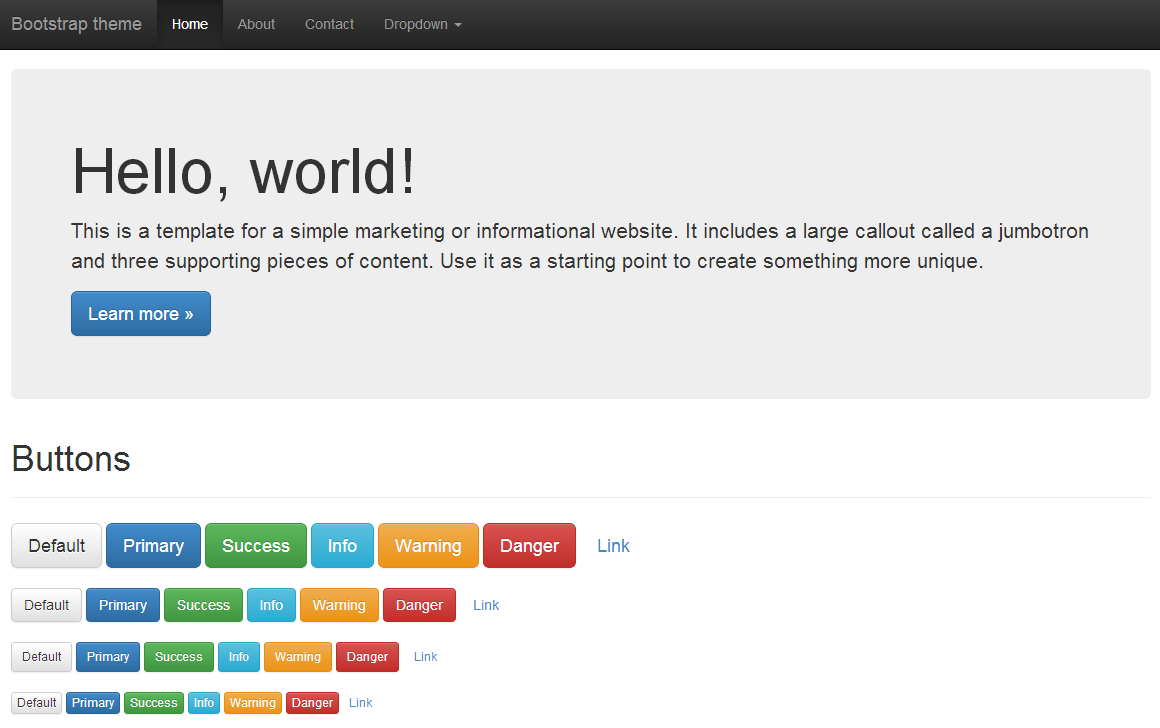
\includegraphics[width=\linewidth]{img/bootstrap.png}
\caption{An example of the look and feel of default Bootstrap}
\end{figure}
Bootstrap~\cite{Bootstrap}, formerly known as Twitter Bootstrap, is a responsive front-end framework. 
It provides CSS classes and JavaScript functions that help developers quickly build a user interface. 
It is highly customizable, and optimized for use on mobile devices. 
The Software Design course has used Bootstrap before, where it allowed students to focus on the functionality of the application and not worry as much about the look and feel. 
Notable features include its grid layout system, which allows complex layouts to be made of HTML divisions with certain CSS classes defining the size and device target. 
Bootstrap then can automatically reflow the layout to be optimal for any screen size.
It also comes with CSS that can be applied to nearly every common HTML element, simplifying the design process and making web page construction much more streamlined than building a UI from scratch. 
This default theme is only the beginning, as users can make or download themes that change the look of default Bootstrap.

\section{Version Control With Git and GitHub}\label{sec:git}
For this project, the course utilized the Git~\cite{Git} software and the GitHub~\cite{GitHub} web service to provide version control capabilities. 
Git was chosen over the previous year's SVN setup due to its more modern feature set including better branch support, faster operations, and a number of other features. 
Using GitHub instead of a local server provided a rich set of collaboration tools and reduced the learning curve by providing a well-designed user interface. 
Each team of students worked on a separate repository, and at the end of the iteration either forked one of them or created a new one for the purposes of aggregating different parts of the last iteration. 
WebStorm also provides an intuitive wrapper around Git, which also helped to dull the learning curve. 
There was some difficulty using the built-in interface to Git; occasionally files deleted from the project were still tracked in Git, and students had trouble reconciling this. 
Git as a system has a steeper learning curve than subversion, and even more experienced users can run into trouble. 
However, when handled properly, Git provides a good system for source code management and the tools built in to the IDE are convenient.


\section{Testing, Continuous Integration and Deployment}\label{sec:CI}
Because the customer for this course is a remote company, we needed a way to show the latest versions of the project from each team. 
We also needed to ensure that the projects passed all the tests, and that teams knew how much of their code was covered by tests. 
To address these issues, we have set up a server to provide continuous integration.

\subsection{Strider}\label{sec:strider}
\begin{figure}[h!]
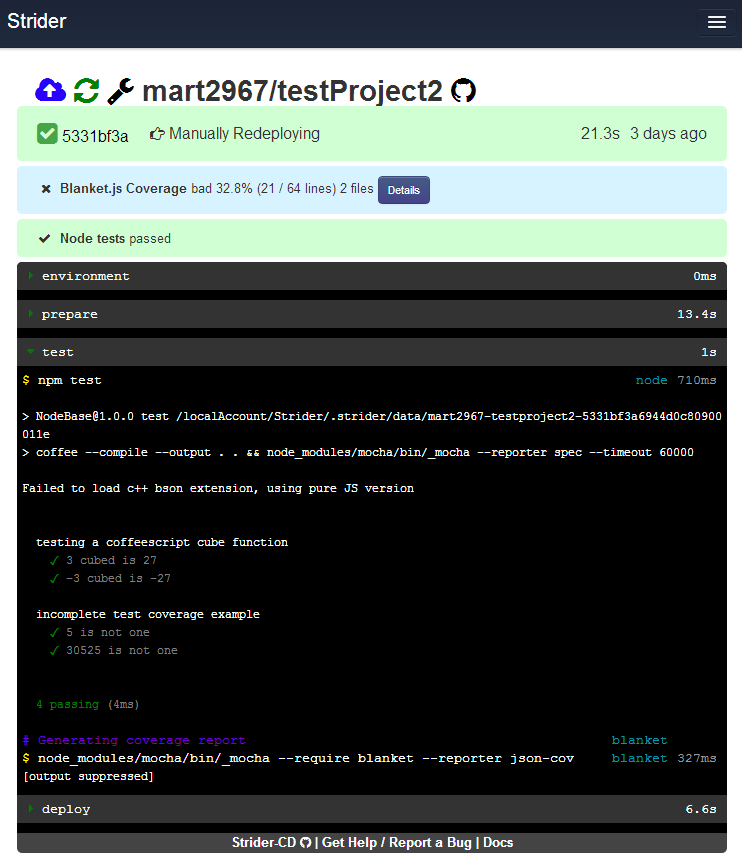
\includegraphics[width=\linewidth]{img/strider_2.png}
\caption{The Strider project dashboard, showing output of Mocha tests}
\end{figure}
Strider~\cite{Strider} is the core of the continuous integration (CI) process. 
It is a software package that manages testing and deployment of repositories. 
When new code is pushed to GitHub, Strider downloads the project, runs the necessary setup scripts, such as \code{npm} and \code{bower}, runs the tests, and computes code coverage data with Blanket, a Node module that supports visual output. 
It then deploys the project to a local web server, from which it can be accessed from anywhere. 
This is quite helpful when trying to present the iteration's progress to the customer. 
Due to the sensitive nature of some of the data used in the project, there are scripts that load private data items such as API keys out of a database on the CI server and pass them directly to Node when starting up the project. 
Strider has very extensible, supporting plugins for custom scripts, deployment to hosting providers, and more.

\subsection{Mocha}\label{sec:mocha}
Mocha~\cite{Mocha} is the testing framework that the students use to verify that their code performed as expected. 
Testing JavaScript code is slightly different than testing other languages. 
It is highly modular, with many components that can be chosen to make a full test suite. 
Mocha itself defines the syntax of the tests, while operations like assertion can be handled by other modules. 
The Blanket module was used for code coverage on the continuous integration server, with students having the option to use that or the Istanbul code coverage module when running tests locally. 
WebStorm ships with enhanced Mocha compatibility, so it was easy to get up and running testing the server. 
Testing the front-end JavaScript, however, was more troublesome due to the lack of Node features like \code{exports} and \code{require}, which, respectively, are needed to make components available to other files, and to access data exported by other files. 
This can be overcome by changing the way in which tests are defined, and the scope in which they are run. 
Possible solutions include using the browser-targeted version of Mocha, or a module like RequireJS to load the right components.



\subsection{Code Coverage}\label{sec:coverage}
\begin{figure}[h!]
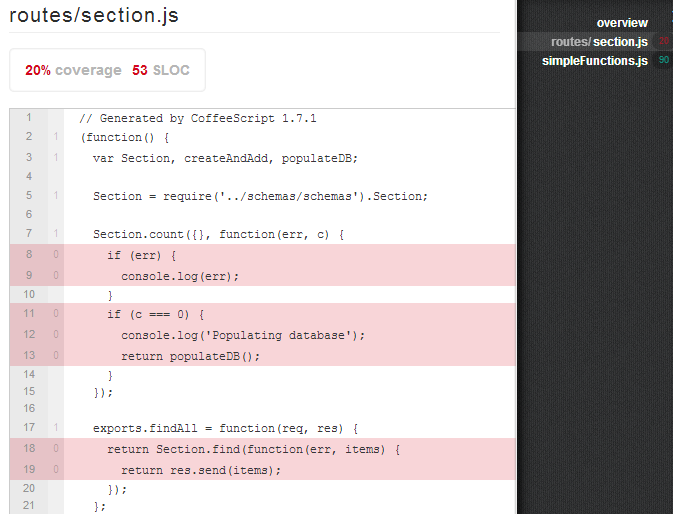
\includegraphics[width=\linewidth]{img/strider_3.png}
\caption{Blanket output, with uncovered lines highlighted}
\end{figure}
Having tests is good, but they are only as good as the amount of code and cases they run through. 
To keep tabs on this data, a code coverage module is used. 
This project uses two different ones, one on the IDE and one on the continuous integration server. 
On the developer's machines, a library called Istanbul~\cite{Istanbul} generates reports showing which lines were tested in each file. 
On the CI server, we use a plugin~\cite{Blanket} for Strider that generates Blanket code coverage reports, which are available right in the page. 
The tests are the same on both ends, it is just the library that has changed. 
This demonstrates the modularity of this development process.


\section{Conclusion}\label{sec:conclusion}
The course is yet ongoing as of this writing, so I will focus on the process rather than the result. 
Students at this point are becoming confident in their ability to work with the tools, and development velocity is increasing. 
However, the learning curve was definitely steep. Students had particular difficulty adopting Backbone.js, partially due to the very granular nature of tasks it performs and the large number of files that result. 
Earlier on, the students were often unsure of what the client should do and what the server should, but this too has been mostly overcome. 
The sheer number of components and understanding the division of responsibilities between them has been one of the most  difficult parts of the course, but the current state of affairs shows signs of continued improvement. 
A key idea that this course imparts is the value of research and the use of libraries; the amount of functionality in this year's and in previous years projects has been greatly increased by the careful selection of plugins and modules. 
Areas that will need improvement include testing of functions that handle HTTP requests, and testing of client-side code. 
The system for generating coverage reports on the development side could be improved, and research into WebStorm's code coverage features is warranted.


%
% The following two commands are all you need in the
% initial runs of your .tex file to
% produce the bibliography for the citations in your paper.
%\bibliographystyle{abbrv}
%\end{thebibliography}




%\bibliography{generic_types}  
% You must have a proper ".bib" file
%  and remember to run:
% latex bibtex latex latex
% to resolve all references
%
% ACM needs 'a single self-contained file'!
%
\bibliographystyle{ACM}
\bibliography{MICS2014NodePaper}
%\printbibliography









\end{document}

%%%%%%%%%%%%%%%%%%%%%%%%%%%%%%%%%%%%%%%%%%%%%%%%%%%%%%%%%%%%%%%%